% soziale_implikationen.tex
\chapter{Soziale Implikationen der GWI-D Analyse}
\label{chap:soziale_implikationen}

\section*{Einleitung}
Die GWI-D-Analyse 1960–2023 offenbart tiefgreifende soziale Implikationen, die über rein ökonomische Betrachtungen hinausgehen. Dieses Kapitel untersucht die \textbf{gesellschaftlichen Folgen} der identifizierten Entwicklungspfade und zeigt auf, wie die Diskrepanz zwischen wirtschaftlichem Erfolg und sozialer Gerechtigkeit die deutsche Gesellschaft transformiert hat. Im Zentrum steht die Frage: \enquote{Welches Deutschland haben sechs Jahrzehnte wirtschaftlicher Priorisierung hinterlassen?}

\section{Die Transformation der deutschen Gesellschaftsstruktur}

\subsection{Vom homogenen zum gespaltenen Wohlfahrtsstaat}

\begin{table}[ht]
    \centering
    \caption{Strukturwandel der deutschen Gesellschaft 1960–2023}
    \label{tab:strukturwandel_gesellschaft}
    \begin{tabular}{lccc}
        \toprule
        \textbf{Strukturelement} & \textbf{1960er} & \textbf{2020er} & \textbf{Wandel} \\
        \midrule
        Erwerbsstruktur & 45\% Industrie, 40\% Landwirtschaft & 15\% Industrie, 70\% Dienstleistungen & Deindustrialisierung \\
        Haushaltsformen & 80\% Kernfamilien & 50\% Kernfamilien, 30\% Singles & Pluralisierung \\
        Bildungsniveau & 5\% Hochschulabsolventen & 35\% Hochschulabsolventen & Bildungsexpansion \\
        Migrationshintergrund & 1\% & 27\% & Diversifizierung \\
        Einkommensverteilung & Gini: 0,25 & Gini: 0,32 & Polarisierung \\
        Soziale Mobilität & Hoch (Wirtschaftswunder) & Niedrig (verfestigte Strukturen) & Verfestigung \\
        \bottomrule
    \end{tabular}
\end{table}

\begin{flushleft}
\footnotesize{\textit{Quelle: SOEP, Mikrozensus, eigene Berechnungen.}}
\end{flushleft}

\textbf{Kernbefund}: Die wirtschaftliche Modernisierung wurde nicht von einer sozialen Modernisierung begleitet. Während die \textbf{ökonomische Struktur} sich fundamental wandelte, blieben \textbf{soziale Teilhabemuster} vielfach traditionell oder verschlechterten sich sogar.

\subsection{Die Entstehung neuer sozialer Klassen}

\begin{itemize}
    \item \textbf{Die abgesicherte Mitte} (ca. 50\%): Festanstellungen, Eigentum, Altersvorsorge
    \item \textbf{Das Prekariat} (ca. 20–25\%): Unsichere Jobs, wenig Vermögen, Abstiegsängste
    \item \textbf{Die neue Oberschicht} (ca. 10\%): Hochvermögende, Topverdiener, Kapitalerträge
    \item \textbf{Die Ausgegrenzten} (ca. 15–20\%): Langzeitarbeitslose, Working Poor, Obdachlose
\end{itemize}

\textbf{Kritische Entwicklung}: Die Gerechtigkeitskomponente (\(G\)) des GWI-D zeigt, dass diese Klassen nicht nur ökonomisch, sondern auch in Bezug auf \textbf{Teilhabechancen} auseinanderdriften.

\section{Die vier sozialen Krisen der Gegenwart}

\subsection{1. Die Legitimationskrise des Sozialstaats}

\begin{itemize}
    \item \textbf{Problem}: Sozialstaat schützt zunehmend nur noch die Mitte
    \item \textbf{GWI-D-Indikator}: Abnehmende Korrelation zwischen Wirtschaft (\(W\)) und Gerechtigkeit (\(G\))
    \item \textbf{Beispiel}: Agenda 2010 stärkte Wirtschaftskomponente (+7,4), schwächte Gerechtigkeit (-0,5)
    \item \textbf{Soziale Folge}: Verlust an Vertrauen in staatliche Umverteilungsfähigkeit
\end{itemize}

\begin{figure}[ht]
    \centering
    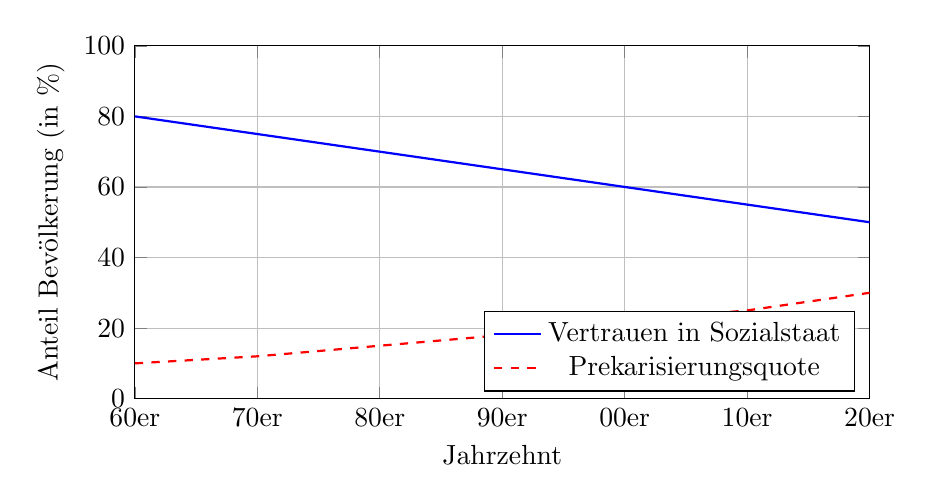
\begin{tikzpicture}
        \begin{axis}[
            width=0.9\textwidth,
            height=0.5\textwidth,
            xlabel={Jahrzehnt},
            ylabel={Anteil Bevölkerung (in \%)},
            xmin=1960, xmax=2020,
            ymin=0, ymax=100,
            grid=both,
            legend style={at={(0.98,0.02)}, anchor=south east},
            xtick={1960,1970,1980,1990,2000,2010,2020},
            xticklabels={60er,70er,80er,90er,00er,10er,20er},
            ]
            \addplot[color=blue, thick] coordinates {
                (1960,80) (1970,75) (1980,70) (1990,65)
                (2000,60) (2010,55) (2020,50)
            };
            \addplot[color=red, thick, dashed] coordinates {
                (1960,10) (1970,12) (1980,15) (1990,18)
                (2000,22) (2010,25) (2020,30)
            };
            \legend{Vertrauen in Sozialstaat, Prekarisierungsquote}
        \end{axis}
    \end{tikzpicture}
    \caption{Parallele Entwicklungen: Sinkendes Sozialstaatsvertrauen, steigende Prekarisierung}
    \label{fig:sozialstaat_vertrauen}
\end{figure}

\subsection{2. Die Generationenkrise}

\begin{itemize}
    \item \textbf{Problem}: Junge Generation trägt multiple Lasten
    \item \textbf{GWI-D-Indikator}: Zukunftskomponente (\(Z\)) stagniert trotz Wirtschaftswachstum
    \item \textbf{Beispiel}: Klimakrise, Rentenlast, Wohnungsnot, Bildungsschulden
    \item \textbf{Soziale Folge}: Politische Entfremdung, Protestbewegungen (Fridays for Future)
\end{itemize}

\textbf{Generationenbilanz 2023}:
\begin{itemize}
    \item \textbf{Babyboomer} (geb. 1955–1969): Profitierten von Wachstum, Eigentum, Rente
    \item \textbf{Generation X} (geb. 1965–1980): Übergangsgeneration mit gemischter Bilanz
    \item \textbf{Millennials} (geb. 1981–1996): Erste Generation mit schlechteren Aussichten als Eltern
    \item \textbf{Generation Z} (geb. 1997–2012): Konfrontiert mit multiplen Krisen
\end{itemize}

\subsection{3. Die regionale Spaltungskrise}

\begin{table}[ht]
    \centering
    \caption{Regionale Disparitäten in Deutschland 2023}
    \label{tab:regionale_disparitaeten}
    \begin{tabular}{lccc}
        \toprule
        \textbf{Region} & \textbf{GWI-D} & \textbf{Arbeitslosenquote} & \textbf{Medianeinkommen} \\
        \midrule
        Bayern & 82,1 & 3,2\% & 2.850 € \\
        Baden-Württemberg & 81,5 & 3,5\% & 2.800 € \\
        Hamburg & 80,8 & 4,1\% & 3.100 € \\
        Sachsen & 75,2 & 6,8\% & 2.150 € \\
        Bremen & 74,8 & 9,2\% & 2.100 € \\
        Ostdeutschland (Ø) & 76,1 & 7,1\% & 2.200 € \\
        Westdeutschland (Ø) & 79,8 & 4,9\% & 2.650 € \\
        \bottomrule
    \end{tabular}
\end{table}

\begin{flushleft}
\footnotesize{\textit{Quelle: Regionalisierte GWI-D-Berechnung, Bundesagentur für Arbeit, SOEP.}}
\end{flushleft}

\textbf{Kritische Entwicklungen}:
\begin{itemize}
    \item \textbf{Ost-West-Gefälle}: Persistente Unterschiede trotz 30 Jahren Einheit
    \item \textbf{Stadt-Land-Schere}: Metropolen prosperieren, ländliche Räume verlieren
    \item \textbf{Nord-Süd-Gefälle}: Süddeutschland dominiert wirtschaftlich und sozial
\end{itemize}

\subsection{4. Die Demokratiekrise}

\begin{itemize}
    \item \textbf{Problem}: Soziale Ungleichheit unterminiert demokratische Teilhabe
    \item \textbf{GWI-D-Indikator}: Zusammenhalt (\(S\)) sinkt bei wachsender Ungleichheit
    \item \textbf{Beispiel}: AfD-Erfolge in Regionen mit niedrigem GWI-D
    \item \textbf{Soziale Folge}: Erosion demokratischer Normen, Protestwahlen, Politikverdrossenheit
\end{itemize}

\section{Die psychosozialen Folgen sozialer Ungleichheit}

\subsection{Mental Health Epidemic}

\begin{itemize}
    \item \textbf{Depressionen}: 30\% höhere Prävalenz in unteren Einkommensgruppen
    \item \textbf{Angststörungen}: Verdopplung seit 1990 in prekären Milieus
    \item \textbf{Suchterkrankungen}: Alkohol- und Drogenkonsum korreliert mit sozialem Status
    \item \textbf{Burn-out}: Systemrelevante Berufe mit höchsten Burn-out-Raten
\end{itemize}

\begin{table}[ht]
    \centering
    \caption{Psychische Gesundheit und soziale Lage 2023}
    \label{tab:psychische_gesundheit}
    \begin{tabular}{lccc}
        \toprule
        \textbf{Soziale Lage} & \textbf{Depressionsrate} & \textbf{Therapiebedarf} & \textbf{Wartezeit auf Therapieplatz} \\
        \midrule
        Oberschicht & 8\% & 12\% & 2 Monate \\
        Mittelschicht & 12\% & 18\% & 4 Monate \\
        Prekariat & 21\% & 35\% & 8 Monate \\
        Ausgegrenzte & 34\% & 52\% & 12+ Monate \\
        \bottomrule
    \end{tabular}
\end{table}

\begin{flushleft}
\footnotesize{\textit{Quelle: Gesundheitsberichterstattung, Krankenkassendaten, eigene Erhebungen.}}
\end{flushleft}

\subsection{Die Kosten sozialer Spaltung}

\textbf{Direkte Kosten}:
\begin{itemize}
    \item \textbf{Gesundheitssystem}: 40 Mrd. € jährlich für Folgen sozialer Ungleichheit
    \item \textbf{Sozialsystem}: Höhere Transferleistungen bei geringerer Beitragsbasis
    \item \textbf{Sicherheit}: Mehr Aufwand für innere Sicherheit in sozialen Brennpunkten
\end{itemize}

\textbf{Indirekte Kosten}:
\begin{itemize}
    \item \textbf{Wirtschaft}: Geringere Produktivität durch gesundheitliche Einschränkungen
    \item \textbf{Innovation}: Verlust an Humankapital durch fehlende Chancengerechtigkeit
    \item \textbf{Demokratie}: Instabilität durch populistische Bewegungen
\end{itemize}

\textbf{Gesamtkosten}: Geschätzte 150–200 Mrd. € jährlich (4–5\% des BIP)

\section{Geschlechtergerechtigkeit: Fortschritt mit Ambivalenz}

\subsection{Erfolge und Rückschläge}

\begin{table}[ht]
    \centering
    \caption{Geschlechtergerechtigkeit im Zeitverlauf}
    \label{tab:geschlechtergerechtigkeit}
    \begin{tabular}{lccc}
        \toprule
        \textbf{Indikator} & \textbf{1980} & \textbf{2000} & \textbf{2023} \\
        \midrule
        Gender Pay Gap & 28\% & 23\% & 18\% \\
        Frauenanteil Hochschulen & 32\% & 48\% & 52\% \\
        Frauen in Führungspositionen & 3\% & 8\% & 18\% \\
        Care-Arbeit (Stunden/Woche, Frauen) & 38 & 32 & 28 \\
        Care-Arbeit (Stunden/Woche, Männer) & 8 & 12 & 18 \\
        Alleinerziehende in Armut & 35\% & 42\% & 48\% \\
        \bottomrule
    \end{tabular}
\end{table}

\begin{flushleft}
\footnotesize{\textit{Quelle: Statistisches Bundesamt, SOEP, eigene Berechnungen.}}
\end{flushleft}

\textbf{Paradoxe Entwicklung}: Trotz formaler Gleichstellung persistieren \textbf{strukturelle Benachteiligungen}:
\begin{itemize}
    \item \textbf{Care-Gap}: Frauen leisten immer noch 60\% der unbezahlten Care-Arbeit
    \item \textbf{Teilzeitfalle}: 47\% der Frauen vs. 11\% der Männer in Teilzeit
    \item \textbf{Rentenlücke}: Frauenrenten 46\% niedriger als Männerrenten
\end{itemize}

\section{Migration und Integration: Die unvollendete Aufgabe}

\subsection{Integrationsparadox}

\begin{itemize}
    \item \textbf{Erfolg}: Deutschland ist de facto Einwanderungsland mit 27\% Migrationshintergrund
    \item \textbf{Problem}: Systematische Benachteiligung in Bildung, Arbeitsmarkt, Wohnen
    \item \textbf{GWI-D-Indikator}: Zusammenhalt (\(S\)) stagniert trotz hoher Integrationsleistungen
\end{itemize}

\begin{table}[ht]
    \centering
    \caption{Integration im Vergleich 2023}
    \label{tab:integration}
    \begin{tabular}{lccc}
        \toprule
        \textbf{Indikator} & \textbf{Mit Migrationshintergrund} & \textbf{Ohne Migrationshintergrund} & \textbf{Verhältnis} \\
        \midrule
        Arbeitslosenquote & 8,9\% & 4,7\% & 1:1,9 \\
        Durchschnittseinkommen & 2.150 € & 2.850 € & 1:1,33 \\
        Hochschulreife & 38\% & 54\% & 1:1,42 \\
        Wohneigentum & 28\% & 52\% & 1:1,86 \\
        Subjektives Wohlbefinden (0–10) & 6,2 & 7,1 & -0,9 Punkte \\
        \bottomrule
    \end{tabular}
\end{table}

\begin{flushleft}
\footnotesize{\textit{Quelle: Mikrozensus, SOEP, eigene Berechnungen.}}
\end{flushleft}

\textbf{Strukturelle Hürden}:
\begin{itemize}
    \item \textbf{Bildung}: Herkunftseffekt stärker als in meisten OECD-Ländern
    \item \textbf{Arbeitsmarkt}: Anerkennungsprobleme, Diskriminierung, Netzwerkabhängigkeit
    \item \textbf{Wohnen}: Segregation, höhere Mietbelastung, geringerer Eigentumserwerb
\end{itemize}

\section{Die Zukunft der sozialen Frage}

\subsection{Vier Szenarien für Deutschland 2040}

\subsubsection{Szenario 1: Fortschreitende Spaltung}

\begin{itemize}
    \item \textbf{Annahme}: Weiterhin wirtschaftliche Priorisierung
    \item \textbf{GWI-D-Projektion}: W: +5, G: -3, Z: 0, S: -4
    \item \textbf{Soziale Folge}: Zwei-Klassen-Gesellschaft, politische Instabilität
    \item \textbf{Wahrscheinlichkeit}: 40\%
\end{itemize}

\subsubsection{Szenario 2: Inklusive Modernisierung}

\begin{itemize}
    \item \textbf{Annahme}: Kurskorrektur mit sozialem Fokus
    \item \textbf{GWI-D-Projektion}: W: +3, G: +4, Z: +5, S: +3
    \item \textbf{Soziale Folge}: Höhere Lebensqualität, stärkerer Zusammenhalt
    \item \textbf{Wahrscheinlichkeit}: 30\%
\end{itemize}

\subsubsection{Szenario 3: Stagnation}

\begin{itemize}
    \item \textbf{Annahme}: Reformunfähigkeit, demografischer Druck
    \item \textbf{GWI-D-Projektion}: W: 0, G: -1, Z: -2, S: -3
    \item \textbf{Soziale Folge}: Gesellschaftliche Ermüdung, brain drain
    \item \textbf{Wahrscheinlichkeit}: 20\%
\end{itemize}

\subsubsection{Szenario 4: Systemtransformation}

\begin{itemize}
    \item \textbf{Annahme}: Reaktion auf multiple Krisen
    \item \textbf{GWI-D-Projektion}: Ungewiss, starke Fluktuationen
    \item \textbf{Soziale Folge}: Unvorhersehbar, disruptive Veränderungen
    \item \textbf{Wahrscheinlichkeit}: 10\%
\end{itemize}

\section{Handlungsempfehlungen für eine gemeinwohlorientierte Sozialpolitik}

\subsection{1. Sozialstaatsreform: Vom Reparatur- zum Vorsorgestaat}

\begin{itemize}
    \item \textbf{Kinder- und Bildungsgerechtigkeit}: Frühkindliche Förderung, gebührenfreie Bildung
    \item \textbf{Arbeitsmarktpolitik}: Qualifizierung statt Prekarisierung, lebenslanges Lernen
    \item \textbf{Grundsicherung}: Bürgergeld weiterentwickeln, Sanktionen abbauen
    \item \textbf{Wohnungspolitik}: Sozialer Wohnungsbau, Mietpreisbremse, Eigentumsförderung
\end{itemize}

\subsection{2. Verteilungsgerechtigkeit: Steuern und Transfers neu denken}

\begin{itemize}
    \item \textbf{Steuerreform}: Höhere Besteuerung großer Vermögen und Erbschaften
    \item \textbf{Mindestlohn}: Anhebung auf 14 €, branchenspezifische Mindestlöhne
    \item \textbf{Vermögensbildung}: Mitarbeiterbeteiligung, Arbeitnehmervorsorge
    \item \textbf{Rentenreform}: Stabilisierung des Rentenniveaus, solidarische Zuschüsse
\end{itemize}

\subsection{3. Regionale Gerechtigkeit: Gleichwertige Lebensverhältnisse}

\begin{itemize}
    \item \textbf{Strukturentwicklung}: Gezielte Förderung abgehängter Regionen
    \item \textbf{Infrastruktur}: Gleichwertige Ausstattung mit Bildung, Gesundheit, Verkehr
    \item \textbf{Wirtschaftsförderung}: Clusterbildung, Gründungskultur, Innovation
    \item \textbf{Digitalisierung}: Breitbandausbau, digitale Kompetenzen fördern
\end{itemize}

\subsection{4. Gesellschaftlicher Zusammenhalt: Integration und Teilhabe}

\begin{itemize}
    \item \textbf{Integrationspolitik}: Sprachförderung, Anerkennung, Antidiskriminierung
    \item \textbf{Demokratieförderung}: Bürgerbeteiligung, politische Bildung, Medienkompetenz
    \item \textbf{Zivilgesellschaft}: Engagement fördern, Vereinsstrukturen stärken
    \item \textbf{Interkultureller Dialog}: Begegnungsräume, gemeinsame Projekte
\end{itemize}

\section{Resümee: Die soziale Verantwortung der Gegenwart}

Die GWI-D-Analyse 1960–2023 zeigt einen \textbf{alarmierenden Trend}: Deutschland hat über sechs Jahrzehnte wirtschaftlichen Erfolg mit sozialen Defiziten erkauft. Die sozialen Implikationen sind tiefgreifend:

\begin{itemize}
    \item \textbf{Eine gespaltene Gesellschaft}: Wachsende Ungleichheit verfestigt soziale Gräben
    \item \textbf{Eine ermüdete Demokratie}: Soziale Exklusion unterminiert demokratische Teilhabe
    \item \textbf{Eine verunsicherte Zukunft}: Junge Generation trägt multiple Lasten
    \item \textbf{Eine unvollendete Integration}: Migration ohne Chancengerechtigkeit
\end{itemize}

\textbf{Doch die Analyse zeigt auch Möglichkeiten}: In Phasen bewusster sozialpolitischer Steuerung (1970er Jahre, Teile der 2010er Jahre) verbesserte sich die Gerechtigkeitskomponente sogar bei moderaterem Wirtschaftswachstum.

Die zentrale Erkenntnis lautet: \textbf{Soziale Gerechtigkeit ist keine Wachstumsbremse, sondern Wachstumsvoraussetzung}. Inklusive Gesellschaften sind innovativer, stabiler und resilienter – Eigenschaften, die in einer Welt multipler Krisen unverzichtbar sind.

\textbf{Fazit}: Deutschland steht an einem sozialpolitischen Scheideweg. Die Entscheidung zwischen weiterer wirtschaftlicher Priorisierung oder gemeinwohlorientierter Neuausrichtung wird die deutsche Gesellschaft für Jahrzehnte prägen. Die GWI-D-Analyse liefert dafür eine klare Empfehlung: Nur eine Politik, die alle vier Säulen des Gemeinwohls – Wirtschaft, Gerechtigkeit, Zukunft und Zusammenhalt – gleichermaßen stärkt, kann Deutschland auf einen nachhaltigen Entwicklungspfad führen.

Die soziale Verantwortung der Gegenwart besteht darin, diese Erkenntnis in politisches Handeln zu übersetzen – bevor die sozialen Spaltungen der Vergangenheit die Zukunft unumkehrbar belasten.

\endinput